\section{Solving Task and Motion Planning Problems}
Solving TAMP problems requires evaluation of
possible courses of action comprised of different combinations of
instantiated action operators. This is particularly challenging
because the set of possible action instantiations (and thus the
branching factor of the underlying search problem) is infinite.
We give a brief overview of SFRCRA-14, a recent approach to TAMP, and
refer the interested reader to the cited paper for further details.
Then, we present a complete algorithm for TAMP that we implemented in
the framework of SFRCRA-14.

\subsection{Preliminaries}
SFRCRA-14 solves TAMP problems by: incrementally
searching for a high-level plan that solves the logical abstraction
of the given TAMP problem; determining a prefix of the plan that has a
motion planning feasible refinement; updating the high-level
abstraction to reflect the reason for infeasibility; and searching for
a new plan suffix from the failure step onwards. This search process
addresses the fundamental TAMP problem: high-level
logical descriptions are lossy abstractions of the true environment
dynamics and thus may not include sufficient information to
determine the true applicability of a sequence of actions.

In general, including geometric properties in the logic-based formulation leads to an
increase in the number of objects representing distinct poses and/or trajectories. For
instance, expressing the fact that a trajectory for grasping \emph{can$_1$} is obstructed by
\emph{can$_3$} from the current pose of the robot would require setting a fluent of the
form \emph{obstructs(can$_3$, pose$_{17877}$, trajectory$_{3219}$, can$_1$)} to true in
the description of the high-level state. In turn, this would require adding
\emph{pose$_{17877}$} and \emph{trajectory$_{3219}$} into the set of objects if they were
not already included. Unfortunately, the size of the abstracted, logic-based state space
grows exponentially with the number of objects, and such an approach quickly leads to
unsolvable task planning problems.

SFRCRA-14 addresses this challenge by abstracting the continuous
action arguments, such as robot grasping poses and trajectories, into
a \emph{bounded} set of symbolic references to potential values. A
\emph{high-level}, or \emph{symbolic}, plan refers to the fixed task
sequence returned by a task planner, and is comprised of these symbolic
references. An \emph{interface layer} conducts plan refinement,
searching for instantiations of continuous values for symbolic
references while ensuring action feasibility.  The resulting process
is able to utilize off-the-shelf task and motion planners while
carrying out the necessary exchange of information in a scalable
manner.

However, this algorithm has two
main limitations: it is not guaranteed to find a solution when
there exists one, and the sets of values from which instantiations
get sampled are object-specific, hand-coded distributions. Since the algorithm
never reduces the set of possible sampled values, its
efficiency degrades as the number of values that get sampled increases. In the next subsection,
we address the first limitation; in the following sections, we address the second.

\begin{figure}[t]
  \centering
    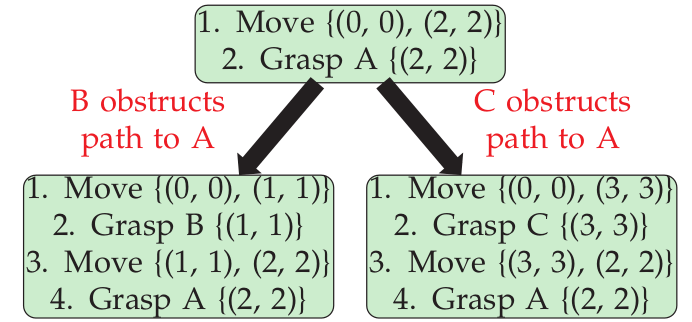
\includegraphics[scale=0.3]{images/ex_prg.png}
  \caption{\small{A simple plan refinement graph for an environment with 3 objects: A,
B, and C. The goal is to grasp object A. Each node maintains a high-level
plan and a set of instantiated continuous values for its symbolic references.
The edges are labeled with errors discovered by the low-level motion planner; these errors are
propagated back up to the task planner for replanning.}}
  \label{fig:prg}
\end{figure}

\subsection{A Complete Algorithm for TAMP}
We introduce a complete algorithm that maintains a \emph{plan
  refinement graph} (PRGraph). \figref{fig:prg} illustrates a simple example.
Every node $u$ in the PRGraph
represents a high-level plan $\pi_u$ and the current state of the search
for a refinement. An edge $(u,v)$ in the PRGraph
represents a ``correction'' of $\pi_u$ for a specific instantiation of
the symbolic references in $\pi_u$. Let $\pi_{u,k}$ be the plan prefix of
$\pi_u$ consisting of the first $k$ actions. Formally, each edge
$e=(u,v)$ is labeled with a tuple $\langle \sigma, k, \varphi \rangle$.
$\sigma$ denotes an instantiation of references for a prefix $\pi_{u,k}$ of
$\pi_u$ such that feasible motion plans have been found for all
previous actions $\pi_{u,k-1}$. $\varphi$ denotes a conjunctive formula
consisting of fluent literals
that were required in the preconditions of the $k^{th}$ action in
$\pi_u$ but were not true in the state obtained upon
application of $\pi_{u,k-1}$ with the instantiation $\sigma_k$.  The
plan in node $v$ (if any) retains the prefix $\pi_{u,k-1}$ and solves
the new high-level problem which incorporates the discovered facts $\varphi_{u,v}$
in the $k^{th}$ state.

The overall search algorithm interleaves the search for feasible
refinements of each high-level plan with the addition into the
PRGraph of new edges and plan nodes using the semantics described
above. This process is described using non-deterministic choices
(denoted using the prefix ``ND'') in
Alg.\,\ref{alg:complete}. Subroutine \textsc{RefineNode} selects a
reference instantiation and attempts to solve the motion planning
problems corresponding to it; subroutine \textsc{AddChild} selects a
reference instantiation and creates a new node that either
incorporates the reason of infeasibility (provided by the
domain-specific subroutine \textsc{GetError}), or makes a random
change in the high-level plan. The latter can be required in some
pathological domains that have dead-ends and where changing the
instantiation of symbolic references for an action has no effect on the
action outcomes.

Different implementations of the non-deterministic choices in
Alg.\,\ref{alg:complete} can capture various search algorithms
with adaptations for handling unbounded branching factors (e.g.,
iterative-deepening with iterative-broadening best first
search). Indeed, SFRCRA-14 can be seen as a greedy depth-first traversal of the
PRGraph. We will show that using trained guided search heuristics with the
PRGraph can lead to performance improvements.

\begin{algorithm}[t]
\begin{small}
  \SetAlgoLined
  \DontPrintSemicolon
  \SetKwFunction{algo}{algo}\SetKwFunction{proc}{proc}
  \SetKwProg{myalg}{Algorithm}{}{}
  \SetKwProg{myproc}{Subroutine}{}{}
  \myalg{Complete TAMP}{
    \nl \For{trial in 1 ...}{
      \nl  \For{j in 1 .. trial}{
        \tcc{\footnotesize Traverse graph of plans, initially with just one plan.}
        \nl $u \leftarrow$ \textsc{NDGetNextNode}(PRGraph)\;
        \nl $\pi \leftarrow$ \textsc{GetHLPlan}($u$)\;
        \nl mode $\leftarrow$ \textsc{NDChoice}\{refine, add child\}\;
        \nl \eIf{mode == refine}{ \textsc{RefineNode}($\pi$, $j$)}{
        \textsc{AddChild}($\pi$, $j$) }}}
  \;
  \setcounter{AlgoLine}{0}
  \myproc{\textsc{RefineNode}($\pi$, $j$)}{
    \nl $\sigma \leftarrow$ \textsc{NDGetInstantiation}($\pi$, $j$)\;
    \tcc{\footnotesize resourceLimit($j$) is monotonically increasing in $j$.}
    \nl  MP, FailedAction, FailedPred $\leftarrow$ \textsc{GetMotionPlan}($\sigma$, $\pi$, resourceLimit($j$))\;
    \nl \If{MP $\ne$ NULL}{
      \nl return success\;
    }
    }\;
    \;
  \setcounter{AlgoLine}{0}
  \myproc{\textsc{AddChild}($\pi$, $j$)}{
    \nl $\sigma \leftarrow$ \textsc{NDGetInstantiation}($\pi$, $j$) \;
    \nl StepNum, FailedPrecon $\leftarrow$ \textsc{GetError}($\sigma$, $\pi$)\;
    \nl mode $\leftarrow$ \textsc{NDChoice}\{error, random\}\;
    \nl \eIf{mode == error} {
      \nl NewState $\leftarrow$ \textsc{Patch}(\textsc{GetStateAt}(StepNum,
      $\pi$), FailedPrecon)\;
    }{
      \nl $\pi\leftarrow$ $\pi$, with an action
      before StepNum replaced $~~~~~~~~~~~$by a random applicable action\;
      \nl NewState $\leftarrow$ \textsc{GetStateAt}(StepNum, $\pi$)\;
    }
    \nl $\pi'\leftarrow$ \textsc{GetClassicalPlan}(NewState)\;
    \nl \textsc{AddNodeToPRGraph}($\sigma$, StepNum, $\pi'$)\;
  }}
\end{small}
\caption{Complete algorithm for TAMP.}
\label{alg:complete}
\end{algorithm}

It is easy to see that the resulting algorithm is complete.

\begin{thm}
If there exists a high-level sequence of actions that 
a) does not revisit symbolic states when using the high-level domain
definition and b) has a motion planning feasible refinement within the scope
of symbol interpretations, then Alg.\,\ref{alg:complete} will find it,
as long as the non-deterministic policies assign non-zero weight to each choice.
\end{thm}

The proof follows easily because if there is a solution, then
the non-deterministic calls can be selected appropriately to find
it. In the next section, we show a specific implementation of \textsc{RefineNode}
based on randomization. Afterward, we show how to train
heuristics that guide the search processes, replacing the non-deterministic choices.



